\section{AFL}

\begin{frame}{AFL}{Algorithme génétique}
  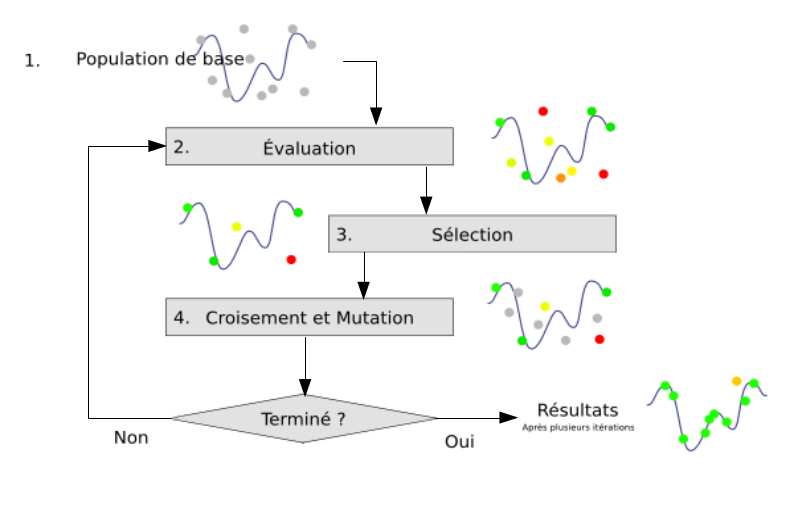
\includegraphics[width=\textwidth]{../medias/schema_genetique.png}
\end{frame}

\begin{frame}{AFL}{Mutations}
  \begin{quote}\Large
  Designing the mutation engine for a new fuzzer has more to do with art than science
  \end{quote}
  \begin{exampleblock}{Stratégies déterministes}
    \begin{itemize}
      \item{bit flip : 1101 0010 devient 1100 0010}
      \item{byte flip : 0xdeadbeef devient 0xde52beef}
      \item{arithmétique simple : 0xdeadbeef devient 0xdeafbeef}
      \item{constantes intéressantes : -1, 256, INT\_MAX, ...}
    \end{itemize}
  \end{exampleblock}
  \begin{exampleblock}{Stratégies aléatoires}
    \begin{itemize}
      \item{unique bit flip}
      \item{remplacement d'un byte aléatoirement ou par un autre intéressant}
      \item{suppression de bloc}
      \item{duplication de bloc via suppression ou insertion}
      \item{memset de bloc}
    \end{itemize}
  \end{exampleblock}
\end{frame}

\begin{frame}{AFL}{Basic Block}
  \begin{figure}
    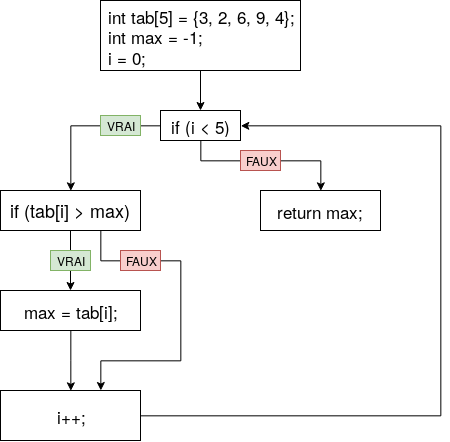
\includegraphics[width=0.65\textwidth]{../medias/BB.png}
  \end{figure}
\end{frame}

\begin{frame}[fragile]{AFL}{Instrumentation}
  L'instrumentation est faite au niveau de chaque basic bloc.
  \begin{lstlisting}
    cur_location = <COMPILE_TIME_RANDOM>;
    shared_mem[cur_location ^ prev_location]++;
    prev_location = cur_location >> 1;
  \end{lstlisting}
  \begin{exampleblock}{Explications}
    \begin{itemize}
      \item Une case du tableau shared\_mem correspond à une flèche du graphe précédent
      \item{Valeur aléatoire pour simplifier l'édition de lien}
      \item{Shift pour différencier A -> B de B -> A, ainsi que A -> A de B -> B}
    \end{itemize}
  \end{exampleblock}
\end{frame}

\begin{frame}{Nouveaux comportements}
  Expliquer comment sont choisis les entrées à garder pour le round suivant
\end{frame}

\begin{frame}{AFL}{Modèle "fork server" (1)}
  \begin{columns}[t]
    \begin{column}{0.49\textwidth}
      \begin{block}{"classique"}
        \begin{itemize}
        \item \lstinline{execve()}
          \begin{itemize}
          \item copie du programme en mémoire
          \item \lstinline{ld-linux.so} charge les librairies partagées
          \end{itemize}
        \item \lstinline{waitpid()}
        \item tout recommencer avec une autre entrée
        \end{itemize}
        \vspace{3.5ex}
      \end{block}
    \end{column}

    \begin{column}{0.49\textwidth}
      \begin{block}{"fork server"}
        \begin{itemize}
        \item \lstinline{execve()} "classique"
        \item programme cible instrumenté
          \begin{itemize}
          \item "pause" avant le \lstinline{main} du programme
          \item \lstinline{fork()} pour copier le processus
          \item \lstinline{waitpid()} pour surveiller les enfants
          \end{itemize}
        \item communication entre alf-fuzz et programme parent avec un \lstinline{pipe}
        \end{itemize}
      \end{block}
    \end{column}
  \end{columns}
\end{frame}

\begin{frame}{AFL}{Modèle "fork server" (2)}
  \begin{columns}[t]
    \begin{column}{0.5\textwidth}
      \begin{center}
        \textbf{"classique"}
      \end{center}

      \bigskip
      \begin{figure}
        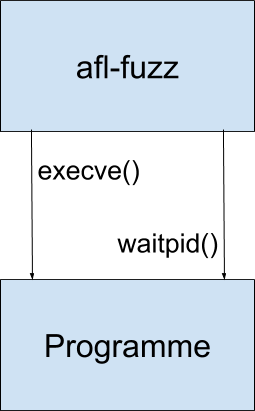
\includegraphics[width=.4\textwidth]{../medias/classique.png}
      \end{figure}
    \end{column}

    \begin{column}{0.5\textwidth}
      \begin{center}
        \textbf{"fork server"}
      \end{center}

      \begin{figure}
        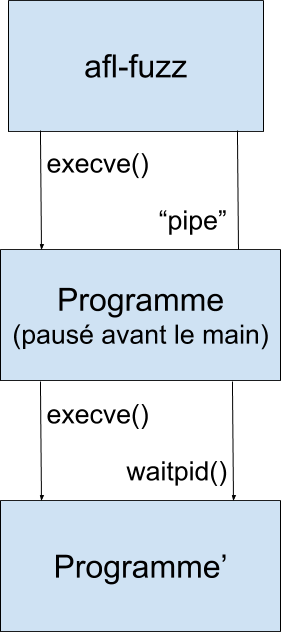
\includegraphics[width=.4\textwidth]{../medias/fork-server.png}
      \end{figure}
    \end{column}
  \end{columns}
\end{frame}
